

\section{Stress and equilibrium}

	\begin{frame}
		\begin{itemize}
		\item We are dealing with different configurations. One configuration is maybe unstressed and the deformed one is. So at the deformed x we should get an equilibrium of stresses and the external loads
		\item Now, the actual stresses at the deformed or current configuration is the Cauchy stress : defined as the force in different directions by the area in different planes
		\item Stresses can also be defined with respect to the initial configuration X			
					
		\end{itemize}

	\end{frame}

	\begin{frame}{Cauchy stress tensor}
		\begin{figure}
			\centering
			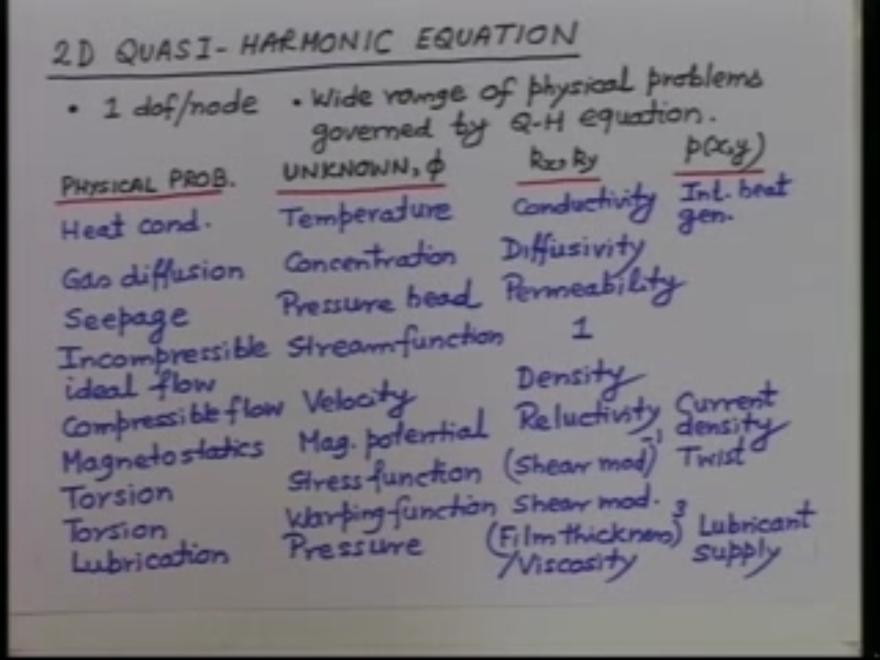
\includegraphics[width=0.5\linewidth]{\pth/continuum/fig7}
		\end{figure}
		At the deformed configuration :
		\begin{itemize}
			\item See two bodies $R_1$ and $R_2$ free body with force acting on them
			\item Imagine the traction vector on a small area element : ${t(n) = \frac{\Delta p}{\Delta a}}$ as lim $\Delta a \rightarrow 0$ where $\Delta p$ is the resultant force
			\item Obviously $t$ and $n$ will depend on the surface it acts on. Here on the right we can see that based on the surface we get opposite forces. (In the negative normal , we will get negative force which is positive in that direction!)

		\end{itemize}
	\end{frame}

	\begin{frame}
		\begin{figure}
			\centering
			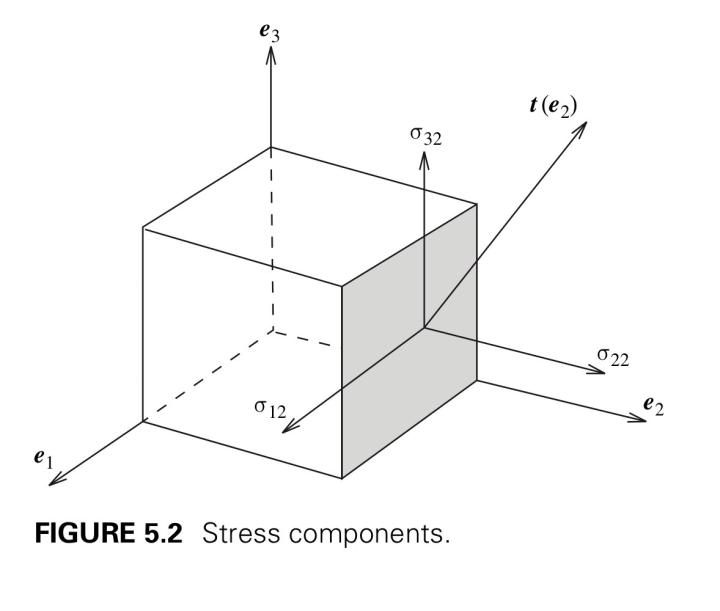
\includegraphics[width=0.5\linewidth]{\pth/continuum/fig8}
		\end{figure}
	
		\begin{itemize}
			\item Let us denote the traction acting on the surface having normals denoted by $e_1, e_2,e_3$
			\item Remember in the other slice we will have an opposite reaction
			\begin{equation}
			\begin{aligned}
			\ve{t(e_1) = \sigma_{1j}e_j} \\\ve{t(e_2) = \sigma_{2j}e_j}\\\ve{t(e_3) = \sigma_{3j}e_j}
			\end{aligned}
			\end{equation}
			\item Or $\ve{t_i = \sigma_{ij}e_j}$
		\end{itemize}
	\end{frame}

	\begin{frame}
		\begin{figure}
			\centering
			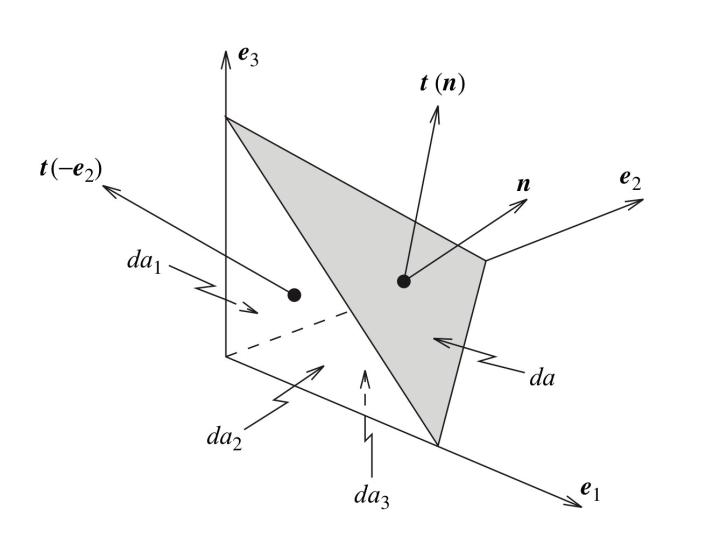
\includegraphics[width=0.5\linewidth]{\pth/continuum/fig9}
		\end{figure}
		
		Now let us look if we take a plane cut of that sphere. Again by context of opposite reactions. All the forces should be equal. So we will use here the concept of equilibrium between the traction vector we have defined in the last slide with respect to some basis and the traction vector defined on the angled plane.
		
		\begin{block}{Equilibrium}
			\begin{equation}
			\ve{t(n)}da + t(\ve{-e_i})da_i + \ve{f}dv = 0
			\end{equation}
			This states that the force vector on the inclined cut should be in equilibrium with the opposite forces defined on the negative sufraces and the body force
		\end{block}
	
	\end{frame}

	\begin{frame}
		\begin{itemize}
			\item  Now the areas (Because they are with defined respect to the basis vectors) can be written as the projection of the inclined area
			\begin{equation}
				da_i = da(\ve{n.e_i})
			\end{equation}
			\item Diving by da we get 
			\begin{equation}
			\ve{t(n)} + t(\ve{-e_i})\frac{da(\ve{n.e_i})}{da} + \ve{f}\frac{dv}{da} = 0
			\end{equation}
			\item $\frac{dv}{da} \rightarrow 0$ 
		\end{itemize}
	\end{frame}